\chapter{Análisis}
\label{chap:analisis}

\lettrine{E}{n} este capítulo se expondrán los requisitos obtenidos tras el estudio de las necesidades que debe cubrir la aplicación
y se elaborarán las historias de usuario.

\section{Requisitos funcionales}
\label{sec:analisis_requisitos_funcionales}

Para la definición de los requisitos funcionales que debe cumplir la aplicación, se ha hecho uso de las historias de usuario.
Esta técnica permite definir los requisitos de una forma más cercana al usuario, ya que se centra en la descripción
de las funcionalidades que este desea que tenga el sistema. Con todo, las historias de usuario obtenidas se muestran en la
Tabla \ref{tab:historias_usuario}.

\bigskip
\begin{table}[H]
	\centering
	\rowcolors{2}{white}{udcgray!25}
	\begin{tabular}{|c|p{11cm}|}
		\rowcolor{udcpink!25}
		\hline
		\small \textbf{ID}                 & \small \textbf{Historia de usuario}                                                                      \\\hline
		\small \textbf{H1} \label{req:hu1} & \small Como usuario quiero poder subir mi propio \textit{dataset} de textos para su perfilado                     \\ \hline
		\small \textbf{H2} \label{req:hu2} & \small Como usuario quiero conocer ejemplos del formato de los \textit{datasets} aceptados                        \\ \hline
		\small \textbf{H3} \label{req:hu3} & \small Como usuario quiero poder seleccionar el algoritmo de perfilado que se va a utilizar              \\ \hline
		\small \textbf{H4} \label{req:hu4} & \small Como usuario quiero poder visualizar los datos obtenidos tras el perfilado                        \\ \hline
		\small \textbf{H5} \label{req:hu5} & \small Como usuario quiero poder ver una lista detallada de cada persona perfilada                       \\ \hline
		\small \textbf{H6} \label{req:hu6} & \small Como usuario quiero poder ordenar la lista de personas por cada uno de los campos perfilados      \\ \hline
		\small \textbf{H7} \label{req:hu7} & \small Como usuario quiero poder saber como funcionan los diferentes algoritmos de perfilado disponibles \\ \hline
		\small \textbf{H8} \label{req:hu8} & \small Como usuario quiero ver el rendimiento de los algoritmos de perfilado disponibles                 \\ \hline
		\small \textbf{H9} \label{req:hu9} & \small Como usuario quiero poder reentrenar los algoritmos con diferentes \textit{datasets}                       \\ \hline
	\end{tabular}
	\caption{Historias de usuario}
	\label{tab:historias_usuario}
\end{table}

A partir de estas historias de usuario se ha obtenido el diagrama de casos de uso
para la interfaz de usuario que se muestra en la Figura \ref{fig:casos_uso}.

\bigskip
\begin{figure}[H]
	\centering
	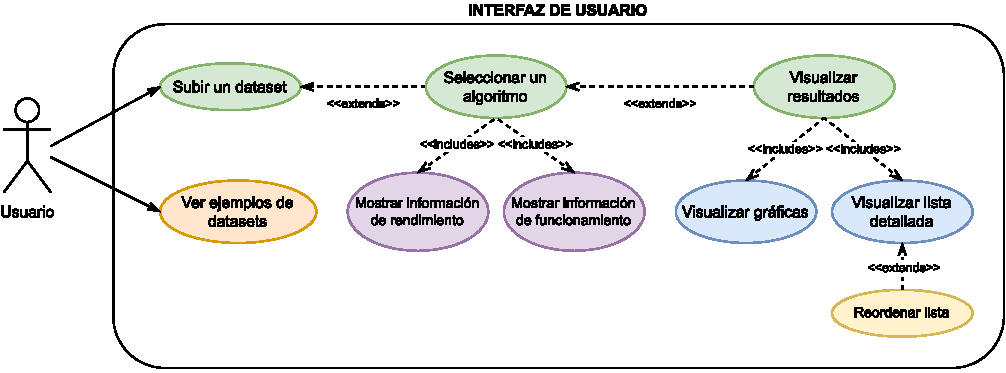
\includegraphics[width=\textwidth]{diagramas/usecases.pdf}
	\caption{Diagrama de casos de uso}
	\label{fig:casos_uso}
\end{figure}

\section{Requisitos no funcionales}
\label{sec:analisis_requisitos_no_funcionales}

Una vez definidas las funcionalidades que debe tener la aplicación, es necesario definir cuales van a ser sus requisitos
no funcionales, esto es, aquellos que están relacionados con cómo debe funcionar la aplicación. En este sentido, a pesar
de que la propia metodología Scrum no contempla la definición de requisitos no funcionales más allá de las historias de usuario,
se ha considerado adaptar esta parte y definirlos por separado para dotarlos de una mayor importancia.
De esta forma, se han determinado los requisitos recogidos en la Tabla \ref{tab:requisitos_no_funcionales}.

\bigskip
\begin{table}[hp!]
	\centering
	\rowcolors{2}{white}{udcgray!25}
	\begin{tabular}{|c|c|p{7.5cm}|}
		\rowcolor{udcpink!25}
		\hline
		\small \textbf{ID}                    & \small \textbf{Requisito} & \small \textbf{Descripción}                                                                      \\\hline
		\small \textbf{RNF1} \label{req:rnf1} & \small Usabilidad         & \small La aplicación debe ser fácil de usar, de forma que cualquier usuario pueda utilizarla sin
		necesidad de tener conocimientos previos sobre el perfilado de autores.                                                                                              \\\hline
		\small \textbf{RNF2} \label{req:rnf2} & \small Escalabilidad      & \small La aplicación debe ser capaz de procesar \textit{datasets} de cualquier tamaño.           \\\hline
		\small \textbf{RNF3} \label{req:rnf3} & \small Portabilidad       & \small La aplicación debe ser capaz de ejecutarse en cualquier sistema, haciendo que
		los usuarios no tengan que preocuparse por el dispositivo que utilizan.                                                                                              \\\hline
	\end{tabular}
	\caption{Requisitos no funcionales}
	\label{tab:requisitos_no_funcionales}
\end{table}
